\chapter{Existing technologies}

In the beginning, I will introduce an existing solution of how to run PHP in a browser. 
The project \cite{Pib} aims to use compiled PHP interpreter into WebAssembly, which allows evaluating a PHP code.
The page has to import a specialized module php-wasm. 
A PHP code is evaluated by writing a specialized script block or manually by JavaScript and API.
PHP can afterward interact with JavaScript using a specialized API.
At first glance, that might be a good enough solution, but they are several parts that can be problematic due to PHP semantics.
The solution doesn't solve globals. 
This is reasonable because this is the server's job, but you are not able to get information about a query part or handling forms without writing a JavaScript code.
The next problem is navigating how a script can navigate to another script without an additional support code which has to be JavaScript.
These problems can be solved by following technologies and their integration.

\section{WebAssembly}

\cite{WebAssembly} is a new code format that can be run in today's browsers. 
It has a compact byte format, and its performance is near to a native code. 
WebAssembly is designed to be a compiling target of popular low-level languages like C or C++ due to its memory model. 
It should be able to support languages with carbage collector in the future. 
The advantage of this format is a similarity with Javascript modules ES2015 after compilation into a machine code. 
This enables browsers to execute it by a JavaScript runtime. 
So its security is as good as a code written in Javascript. 
Because of the same runtime, WebAssembly can call Javascript and vice versa.

\cite{Threads} support is currently discussed nowadays and appears to be realistic.
After all, new versions of Google Chrome experiments with true multi-threading support despite of the chance of vulnerability.
A replacement of multi-threading can be web workers refered in \cite{WebWorkers} article.
The workers limitation is comunication with UI thread only by messages.

Despite supporting to run WebAssembly in a browser, the browser cannot load it as a standard ES2015 module yet.
WebAssembly JavaScript API was created in order to be able to load a WebAssembly to a browser using JavaScript.

\section{Mono}

Mono is a .NET runtime that aims to mobile platforms. 
Recently, they started to support \cite{compilation} into WebAssembly.
This support allows executing CIL inside browsers.
The compilation has two modes.
The first one is compilation Mono runtime with all using assemblies.
The second only compile Mono runtime, which then can execute .dll files without further compilation of them into WebAssembly.
A consequence of these compilations into WebAssembly is enabling to call Javascript and WebAPI from .NET.

\section{Blazor}

Blazor is a framework that provides a convenient way how to write dynamic web pages using CSharp.
Blazor platform is divided into two \cite{Hosting_models} which have different approaches to creating web applications. 
The first one is referred to as Blazor Server App and has a similar methodology to a standard website written in PHP.
An interesting innovation is SignalR which is a communication protocol between the server and a client.
However, this thesis uses the second model, which Microsoft refers to as Blazor WebAssembly App enabling offline support after loading the app into a browser.

\subsection{Blazor WebAssembly App}
From now on, I will use Blazor App to refer Blazor WebAssembly App.
Blazor App can be divided into two parts.
The first part serves the main WebAssembly application and its additional resources, which can be requested during runtime.
The second part is WebAssembly wrapped together with an additional user code.
The division enables to choose of a place for the implementation of business logic.
If there is a bad connection, we can move the majority of business logic to the client and use the server for connection to a database; otherwise, we can use the client only for rendering the page. It consists of the following components. 
Kestrel with ASP.NET libraries provides the server part of an application.
Mono runtime compiled to WebAssembly runs CSharp code inside a browser.
WebAssembly is essential for being able to interact with DOM and JavaScript using CSharp without an additional plugin, which was necessary for older technologies like Microsoft Silverlight.
Blazor's libraries provide constructs for manipulation with DOM and WebAPI together with rendering the page and JavaScript interop.
And there is a user's code that using the libraries for creating dynamic pages with CSharp.
A better imagination, how the app is situated on the client-side, can be represented by the figure \ref{img01:wasm} copied from \cite{Glick2018}.

\begin{figure}[H]\centering
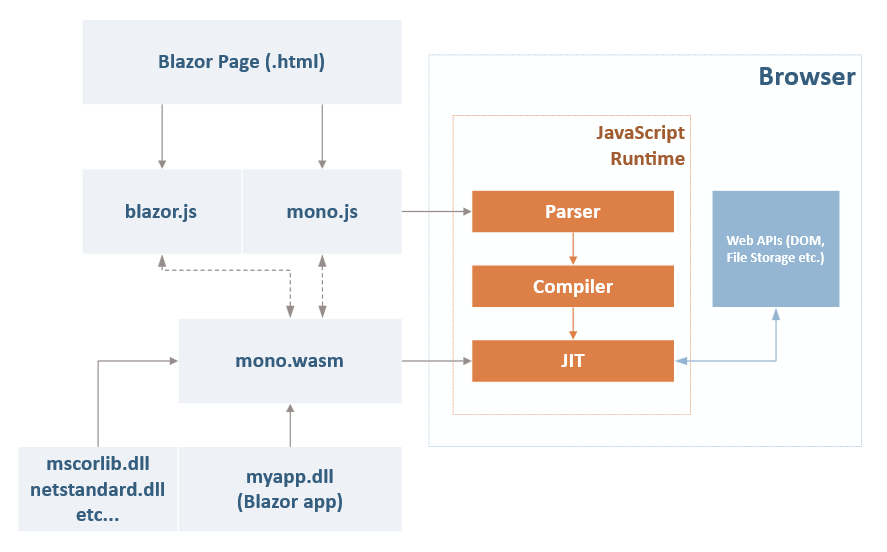
\includegraphics[width=140mm, height=100mm]{./img/BlazorExecution}
\caption{Running a Blazor WebAssembly App on client-side.}
\label{img01:wasm}
\end{figure}

Technical details of interop with a browser are one part of the Blazor App.
The main part is the architecture of the libraries.
A common approach how to create a page is using the markup language Razor.
There already exists Razor in standard ASP.NET website where .cshtml extensions consist of this markup.
Unfortunately, the markup used in BlazorApp has the same name.
From now on, I will use Razor for the markup language, which is the content of .razor files in Blazor App.
Because interleaving HTML with other languages turns out to be helpful, the Razor uses special characters to identify CSharp code in HTML and convert it to rich content pages.
A significant purpose of Razor is for generating CSharp structures, which represent parts of a page, during compilation time.
These structures have a complex interface for rendering a page, so the markup is there in order to free users using a complicated mechanism for putting a page together.

Blazor introduces a Component that can represent a whole page or the part of it.
Components can be arbitrarily put together in order to form the desired page.
They can have different purposes. For example, a Router takes care of routing the right page whenever the navigation is triggered.
Alongside components, a dispatcher supplies additional services like logger to components when they are creating.
The last item, which is not used transparently, is a WebAssemblyHost builder.
The builder configures the application and prepares the renderer used by components to render their content.

Balzor presents its own virtual DOM to reduce changing a DOM directly in a browser to its demanding performance.
A component works with RenderTreeBuilder, which provides an interface for adding content to the virtual DOM.
The usage of RenderTreeBuilder is complex due to Blazor's diff algorithm, which is used afterward.
RenderTreeBuilder is just a superstructure over Renderer, which is responsible for updating the page.
The diff algorithm is used to minimize the browser's DOM  update after all components used RenderTreeBuilder to render their content.
This algorithm used sequence numbers for parts of HTML to identify modified sections.
Sequence numbers respond to an order of RenderTreeBuilder's instructions in the source code.
A benefit of this information is detecting loops and conditional statements to generating smaller updates of DOM.  
It follows the browser's DOM update, which is executed by Blazor's JavaScript support code called through Mono runtime.

The process of bootstrapping the Blazor App to a browser follows these steps. 
Kestrel gets a request for a page that is contained in Blazor App. 
The server responses with the index.html page, which contains references to JavaScript support code (This code is referred to as blazor.js and mono.js in the figure \ref{img01:wasm}) responsible for loading and running the runtime with the application part.
The runtime runs the application using the Main method in Blazor App.
The remaining interactions are maintained by event handling.
I distinguish two types of events.
The first type is navigation.
The \cite{navigation} can be triggered by an anchor, form, or filling up the URL bar.
The URL bar is handled separated by a browser.
JavaScript can influence the remainings elements.
Blazor App handles only an anchor by.
After clicking on an anchor, predefined methods in blazor.js try to invoke navigation handler in Blazor App using a Mono WebAssembly gateway.
A user can modify this handler, but a specialized component Router implements a default behavior.
The Router finds out all components, which implements an IComponent interface, by a reflection and tries to render the page according to path matching RouteAttribute of a component.
The navigation can be redirected to the server if there is no match.
The second type is events invoked by UI like onchange. These event's callbacks call right CSharp callbacks thanks to RenderTreeBuilder, connecting CSharp callback with element's event.

\section{Peachpie}

\cite{Peachpie} is a modern compiler based on Roslyn and Phalenger project.
It allows to compile PHP into a .NET assemmbly, which can be executed alongside standard .NET libraries.
Peachpie introduces several structures representing states, scripts, and variables of PHP written in Csharp.
First of them is a context representing one request to PHP code.
The context consists of super globals, global variables, declared functions, declared and included srcipts.
A possibility of saving the context and using it later is a major advantage used in the solution.
The context can be also consider as a configuration of comming script's execution.
Every information about a request can be arrange to mock every situation on server-side.
The compiler offers dedicated type of assembly for PHP libraries.
Using this assembly can add addition functions, which can provides a extra nonstandard functinality as an interaction with a browser.
Another advantage of the compiler is a great interoperability between PHP and .NET.
An option to work with Csharp objects, attributes and calling methods will become crutial for achieving advanced interaction between Blazor and PHP.

However there are limitations following from differences of the languages and the stage of development.
Availability of PHP extensions depend on binding these function to CSharp code giving equivalent results, even more a time and memory complexity together with supporting this code in Blazor can be tricky.
The previous mentioned interoperability has limits as well.
Csharp constructs like structs and asynchronous methods are undefined in PHP.

\section{PHP}

\change[inline]{TODO: Specification(paradigm, dynamic language, HTML interleaving, Globals, No async functions)}
\change[inline]{TODO: Classic web page in php (Forms, HTML interleaving, Front controller, Database, Sessions, HTTP, JavaScript??)}
